\chapter{Simple Prototype}
\section{Introduction}
In this chapter we will discuss about a simple prototype we made using the design from the pseudonym system in chapter 4. We will describe different parts of the system and how end user perceives it.
\section{Design}
The system is based on the design given in Chapter 4. 
\begin{figure}[h]
	\centering
	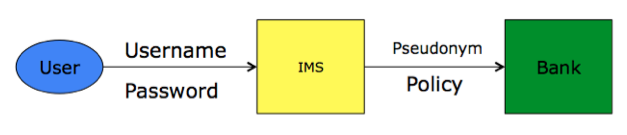
\includegraphics[width=\textwidth]{figures/Pseudonym}
	\caption{Prototype Design}
	\label{fig:Pseudonym}
\end{figure}
For end user it doesn't change anything. End user authenticates to the IMS and then IMS creates a pseudonym for the user. This pseudonym is then used by the bank for providing the services to the customer.
\section{Authentication}
User authentication happens as follows:
\begin{itemize}
	\item User goes to the bank login page.
	\item User puts his credentials in the login system.
	\item User credentials are verified by IMS and then user is redirected to his account page.
	
\end{itemize}